\section{Results}

As PET has been optimized by a genetic inspired algorithm, it is likly to perform very well on the data sets it
has been optimized for. When such training is done, a controll test is needed in order to verify that the result
is good for the general problem solved, not only the specific instances used for training.

\subsection{Training}

The training sets:
\begin{figure}
\centering
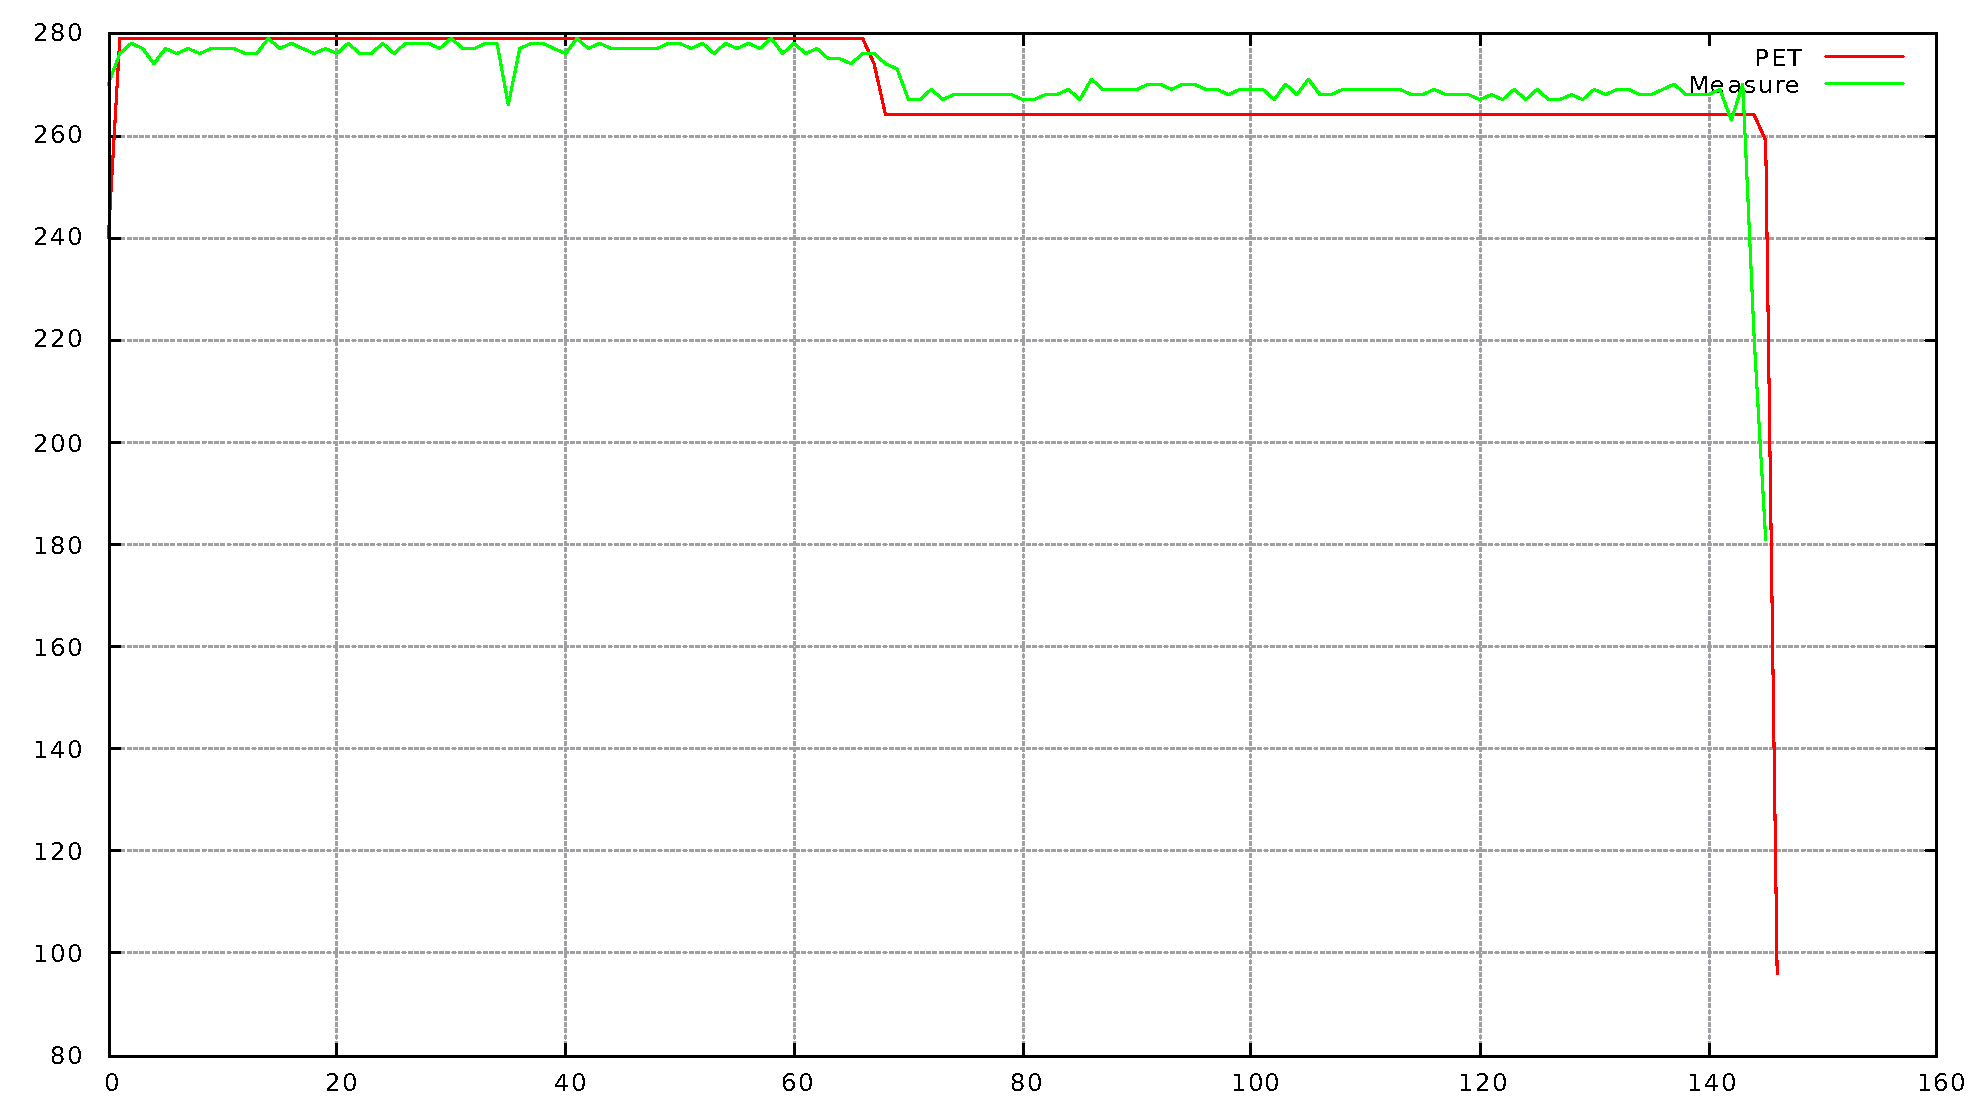
\includegraphics[width=\textwidth]{figs/trend-training.pdf}
\caption{Overlay of PET training results (red) and training data (green)}
\label{fig:trend-training}
\end{figure}

\subsection{Controll}

How well did we do it on different real world test sets.
